%360 degree two lines 4 angle split
\documentclass[tikz,border=10pt]{standalone}
\usepackage{tikz}
\usetikzlibrary{angles,quotes,calc} % Add this for angle labels

\begin{document}

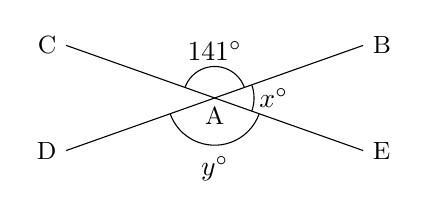
\begin{tikzpicture}[scale=1]
    % Define the points of the cube
    \coordinate (A) at (0,0);
    \coordinate (B) at ($(A)+(19.5:2cm)$); 
    \coordinate (C) at ($(A)+(160.5:2cm)$); 
    \coordinate (D) at ($(A)+(199.5:2cm)$); 
    \coordinate (E) at ($(A)+(340.5:2cm)$); 

    % Draw the visible edges of the cube
    \draw (A) -- (B);
    \draw (A) -- (C);
    \draw (A) -- (D);
    \draw (A) -- (E);
    
    % Draw the angle between lines
    \pic [draw, "$141^{\circ}$", angle eccentricity=1.5, angle radius=0.4cm] {angle = B--A--C};
    \pic [draw, "$x^{\circ}$", angle eccentricity=1.5, angle radius=0.5cm] {angle = E--A--B};
    \pic [draw, "$y^{\circ}$", angle eccentricity=1.5, angle radius=0.6cm] {angle = D--A--E};

    % Place the labels with smaller font size
    \node at (A) [below,font=\small] {A};
    \node at (B) [right,font=\small] {B};
    \node at (C) [left,font=\small] {C};
    \node at (D) [left,font=\small] {D};
    \node at (E) [right,font=\small] {E};
    
\end{tikzpicture}

\end{document}